\section{Ziel}
In diesem Versuch soll die Wällenlänge des verwendeten Lasers bestimmt werden, sowie der Brechungsindex von Luft.
\section{Theorie}
\subsection{Interferenz und Kohärentes Licht}
Das Michelson-Interferometer basiert auf dem Prinzip der Interferenz.\\
Licht ist ein elektromagnetische Welle und breitet sich nach Maxwell in der allgemeinsten Form für die elektrische Feldstärke ,
\begin{equation}
    \vec{E}(x,t)=\vec{E}_0\left(1+\cos (kx-wt-\gamma)\right),
\end{equation}
wobei $k=\frac{2\pi}{\lambda}$ die Wellenzahl, $\lambda$ die Wellenlänge, $w$ die Kreisfrequenz und $\gamma$ der Phasenwinkel ist.
Hierbei gilt das Superpositionsprinzip. Da die elektrische Feldstärke von Licht im allgemeinen nicht 
einfach zu messen ist, greift man auf die Inetensität $I$ zurück,
\begin{equation}
    I=\text{const}|\vec{E}|^2.
\end{equation}
Bei der überlagerung mit einer zweiten Welle folgt darfür,
\begin{equation}
    I_{\text{ges}}=2\text{const}\vec{E}_0(1+\cos (\gamma_2-\gamma_1)).
\end{equation}
Man sieht, dass für den hinteren Teil, die Gleichung für ein ungerades Vielfaches von $\pi$ verschwindet.\\

Zudem muss noch hinzugefügt werden, dass eine Interferenz für Licht aus zwei verschiedenen quellen im Allgemeinen nicht möglich ist.
Dies folgt aus der Entstehung des Lichtes. Eine elektrische Welle wird demnach von einem Atom ausgegebe, wenn es in den Grundzustand zurückgeht.
Wird diese Welle über einen genügend großen Zeitraum gemittelt, so verschwindet der hintere Interfrenzterm.
Man spricht von inkohärentem Licht.\\
Besitzt das Licht en festes $k, w$ und $\gamma$ so spricht man von Kohärentem Licht.\\


Es ist allerdings möglich eine Interferenz des Lichtes aus einer Quelle zu beobachten, Hierfür wird
der Lichtstrahlt aufgeteilt und zu einem späteren zeitpunkt wieder zusammengeführt.
Da die beiden Lichtstrahlen verschiedene lange Wege durchlaufen sind, führt die Phasendifferenz zur Interferenz.
Ob eine Interferenz überhaut zu beobachten ist ist dabei von der Kohärenzlänge $l$ abhängig.
So folgt für den Zusammenhang zwischen Interferenmaxima $N$, Wellenlänge $\lambda$ 
und Kohärenzlänge $l$
\begin{equation}
    l=N\cdot\lambda
\end{equation}

\subsection{Das Michelson-Interferometer}
Hierbei wird sich die Teilung des Lichtes zu nutzen gemacht. Ein semipermaeables MAterial teilt den Lichtstrahlt.
Dabei geht ein teil des Lichtes durch den Strahl, während ein anderer Teil abgelenkt wird.
Beide Strahlen laufen zu einem Spiegel (hier $S_1$ und $S_2$) und werden zurückgeworfen, sodass sie sich am Punkt $P$
wieder treffen und gemeinsam zum Detektor $D$ gelangen können.
Um nun eine Interferenz zu beobachten müssen beiden Strahlen koärebt sein.
Um dies zu erreichen, werden die Strecken $\bar{S_1P}$ und $\bar{S_2P}$ gelcih gewählt. Zusätzlich stelle amn ene Kompensationsplatte 
in den Weg zwischen $P$ und $S_2$, welche die optische Weglänge der Strahlen ausgleicht, weil der Strahl zu $S_1$ die Platte dreimal druchläuft,
während der Strahl zu $S_1$ sie nur zweimal durchläuft.\\
\begin{figure}
    \centering
    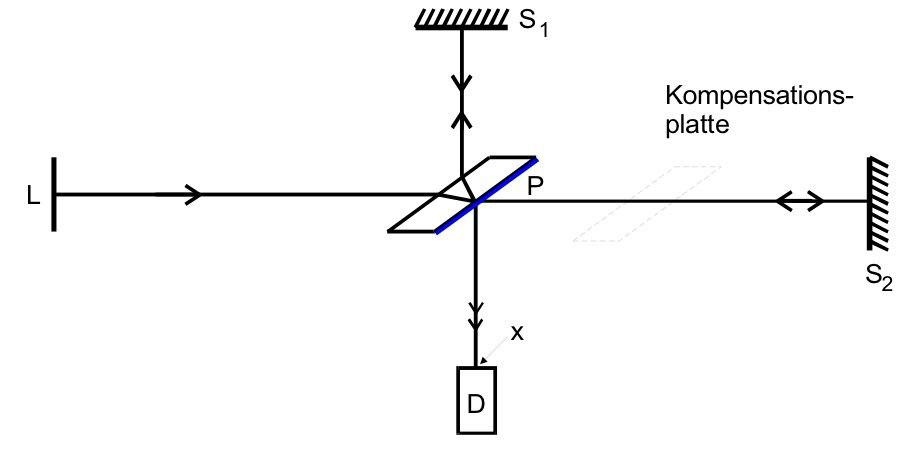
\includegraphics[width=0.5\textwidth]{bilder/s.jpg}
    \caption{Schematischer Aufbau Michelson-Interferometer \cite[9]{anleitung}}
\end{figure}
Nun kann über die Verschiebung $\Delta d$ der Spiegel die Inetensität der Interfernezmuster am Ort $D$
varrieren. Für die Wellenlänge $\lambda$ folgt dardurch
\begin{equation}
    \Delta d = z \cdot \frac{\lambda}{2}
\end{equation}
wobei $z$ für die Anzahl der beobachteten Interferenzmaxima steht.
Sind die Abstände zwischen $P$ und den Spiegel gleich, so ergibt sich ein Gangunterschied von $\frac{\pi}{2}$.\\
Das Ergebnis bei $D$ ist eine destruktive Interferenz.


Neben der Möglichkeit die Wegstrecke zu varrieren kann auch der Brechungsindex nach $n+\Delta n$ variiert werden. 
Dies kann durch ein Medium der Länge $b$ realisiert werden.
Für den Wegunterschied folgt nun
\begin{equation}
    \Delta d =b\cdot \Delta n.
\end{equation}
Für die Beobachtungen bei $D$ folgt
\begin{equation}
    b\cdot \Delta n = \frac{z\lambda}{2}
\end{equation}
\begin{figure}
    \centering
    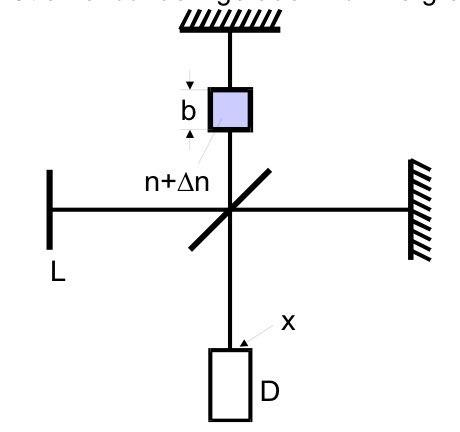
\includegraphics[width=0.4\textwidth]{bilder/n.jpg}
    \caption{Schematischer Aufbau zur Messung von Brechnungsindexunterschieden \cite[5]{anleitung}}
\end{figure}
\label{sec:theorie}